\chapter{Symbolic Block Linear Algebra}

In mathematics literature, it is common practice to represent matrices as being broken up into blocks or sub-matrices.
For example if $A$, $B$, $C$ and $D$ are matrices given by:
\begin{equation}
	A = \begin{bmatrix} 
		A_{1,1} & \ldots & A_{1,m} \\
		\vdots & & \vdots \\
		A_{n,1} & \ldots & A_{n,m}
	\end{bmatrix}
	\;\;\;\;
	B = \begin{bmatrix} 
		B_{1,1} & \ldots & B_{1,q} \\
		\vdots & & \vdots \\
		B_{n,1} & \ldots & B_{n,q}
	\end{bmatrix}	
	\;\;\;\;
	C = \begin{bmatrix} 
		C_{1,1} & \ldots & C_{1,m} \\
		\vdots & & \vdots \\
		C_{r,1} & \ldots & C_{r,m}
	\end{bmatrix}
	\;\;\;\;
	D = \begin{bmatrix} 
		D_{1,1} & \ldots & D_{1,q} \\
		\vdots & & \vdots \\
		D_{r,1} & \ldots & D_{r,q}
	\end{bmatrix}			
\end{equation}
Where, critically, $A$ and $C$ have the same width (namely $m$) as do $B$ and $D$ (width $q$).
Additionally, $A$ and $B$ have the same height (in this case $n$), as do $C$ and $D$ (height $r$).
Then they can be ``glued'' together into a single  $\boldsymbol{(2 \times 2)}$ \textbf{block matrix} $M$.
Notationally, we write these matrices as elements of $M$ but we \emph{interpret} $M$ as a sort of concatenation of the
sub-matrices.
\begin{equation}
	M= \left[
		\begin{array}{c|c}
			A & B \\
			\hline
			C & D \\
		\end{array}
	\right] = \left[
		\begin{array}{ccc|ccc}
			A_{1,1} & \ldots &A_{1,m} & B_{1,1} & \ldots & B_{1,q} \\
			\vdots & & \vdots & \vdots & & \vdots \\
			A_{n, 1} & \ldots & A_{n, m} & B_{n,1} & \ldots & B_{n,q} \\
			\hline
			C_{1, 1} & \ldots & C_{1, m} & D_{1,1} & \ldots & D_{1,q} \\
			\vdots & & \vdots & \vdots & & \vdots \\
			C_{r,1} & \ldots & C_{r,m} & D_{r,1} & \ldots & D_{r,q} \\
		\end{array}
	\right]
\end{equation}


So $M$ is actually a $(n+r) \times (m+q)$ matrix but we write it as a $2 \times 2$ \emph{block} matrix.
Within an individual block, there is a one-to-one correspondence from the entries of $M$ to the entries of a sub-matrix 
(shifted by some offset).
In the above example, elements of $B$ would have an offset of $(0,m)$ since $B_{i,j}$ corresponds with $M_{i+0, j+m}$.


There is no reason to stop at combining 4 matrices into a $2 \times 2$ block matrix.
We can take a set of matrices $A_{i,j}$ and combine them into an $\boldsymbol{(n\times m)}$ \textbf{block matrix}:
\begin{equation*}
	M = \left[ \begin{array}{c|c|c|c}
		A_{1,1} & A_{1,2} &\ldots & A_{1,m} \\
		\hline
		A_{2,1} & A_{2,2} & \ldots & A_{2,m} \\
		\hline
		\vdots & \vdots & & \vdots \\
		\hline
		A_{n,1} & A_{n,2} & \ldots & A_{n,m}

	\end{array}\right]
\end{equation*}


In the $2\times 2$ case, we enforced that for example the height of $A$ was the same as the height of $B$.
Similarly, here it is an important condition that these partitions are divided by \emph{unbroken} horizontal and vertical lines.
Formally, for each sub-matrix $A_{i,j}$ in $M$ then $A_{i,j}$ is a $s_i \times t_j$ matrix for strictly positive integer sequences $\{s_i\}_{i=1}^n$ and $\{t_j\}_{j=1}^m$ common to all sub-matrices.
As before we interpret the block matrix as a concatenation of its sub-matrices.
Thus $M$ is a $n\times m$ block matrix but a $\left( \sum_{i=1}^n s_i \right) \times \left( \sum_{j=1}^m t_j \right)$
block matrix.


Clearly block matrices are at the very least a convenient notation but they also have considerable practical applications as well.
For example when multiplying large matrices, block matrices can be used to improve cache complexity \cite{lam1991cache}.
Additionally, in some cases, when a sub-matrices are known to have a nice properties, many optimizations can arise.
For example to invert what is known as a \emph{block diagonal matrix}, one can invert each block individually:
\begin{equation}
	\begin{bmatrix}
		A_1 & 0 & \ldots & 0 \\
		0 & A_2 & \ddots & \vdots \\
		\vdots & \ddots & \ddots & 0 \\
		0 & \ldots & 0 & A_n \\
	\end{bmatrix}^{-1}
	=
	\begin{bmatrix}
		{A_1}^{-1} & 0 & \ldots & 0 \\
		0 & {A_2}^{-1} & \ddots & \vdots \\
		\vdots & \ddots & \ddots & 0 \\
		0 & \ldots & 0 & {A_n}^{-1} \\
	\end{bmatrix}
\end{equation}


\begin{figure}[ht]
	\caption[Possible block overlaps of $2 \times 2$ block matrices.]{There are 9 possible permutations. 1x (a) 2x (b) 2x (c) 4x (d)}
	\label{MatAdditionPermutations}
	\begin{subfigure}[b]{0.24\textwidth}
		\caption{}
		\begin{equation*}
			\left[ \begin{array}{c|c}
				\; & \; \\
				\hline
				& \\
			\end{array}\right]
		\end{equation*}
	\end{subfigure}
	\begin{subfigure}[b]{0.24\textwidth}
		\caption{}
		\begin{equation*}
			\left[ \begin{array}{c|c}
				\; & \; \\
				\hline
				& \\
				\hline
				& \\
			\end{array}\right]
		\end{equation*}
	\end{subfigure}
	\begin{subfigure}[b]{0.24\textwidth}
		\caption{}
		\begin{equation*}
			\left[ \begin{array}{c|c|c}
				\; & \; & \;  \\
				\hline
				& \\
			\end{array}\right]
		\end{equation*}
	\end{subfigure}
	\begin{subfigure}[b]{0.24\textwidth}
		\caption{}
		\begin{equation*}
			\left[ \begin{array}{c|c|c}
				\; & \; & \; \\
				\hline
				& \\
				\hline
				& \\
			\end{array}\right]
		\end{equation*}
	\end{subfigure}
\end{figure}

Although block matrices are commonly used with fixed values for bounds.
Computer algebra has unsatisfactory structures to represent these when the bounds between blocks are symbolic.
For example, the sum of $2 \times 2$ block matrices, naively leads to 9 possible cases of overlapping regions depending on
the relationship between horizontal and vertical boundaries between blocks.
In this chapter we will show a method using hybrid functions to avoid this case based approach for both addition
and multiplication of matrices.
First we introduce some notation that will be used frequently over the next 3 chapters.

%%%%%%%%%%%%%%%%%%%%%%%%%%%%%%%%%%%%%%%%%
%
% INTERVALS
%
%%%%%%%%%%%%%%%%%%%%%%%%%%%%%%%%%%%%%%%%%

\section{Oriented Intervals}

\begin{definition}
	Given a totally ordered set $(X, \leq)$ \emph{(and with an implied strict ordering $<$)}, 
	for any $a,b \in X$, an \textbf{interval between $\boldsymbol{a}$ and $\boldsymbol{b}$} 
	is the set of elements in $X$ between $a$ and $b$, up to inclusion of $a$ and $b$ themselves. 
	Formally:
	\begin{equation} 
	\begin{array}{cc}
		{[a,b]}_X =  \{ x \in X \;|\; a \leq x \leq b \} \\
		{[a,b)}_X =  \{ x \in X \;|\; a \leq x < b \} \\
		{(a,b]}_X =  \{ x \in X \;|\; a < x \leq b \} \\
		{(a,b)}_X =  \{ x \in X \;|\; a < x < b \}
	\end{array} 
	\end{equation}
	When context makes $X$ obvious or the choice of $X$ is irrelevant, we shall omit the subscript.
\end{definition}

It should be noted that when $b$ is less than $a$, $[b,a]$ is the empty set. 
In terms of idempotency, the bounds determine whether or not an interval will be empty.
$[a,a]$ which contains $a$ and all points equivalent to $a$ while $(a,a)$, $(a,a]$, and $[a,a)$ are all empty sets.
As intervals are simply sets, they can naturally be interpreted as hybrid sets.
If $a \leq b \leq c$, for intervals then we have $[a,b) \oplus [b,c) = [a,c)$.
In this case, $\oplus$ seems to behave like concatenation but this is not always true.
If instead we had $a \leq c \leq b$ then $[a,b) \oplus [b,c) = [a,b)$.

\begin{equation}
	[a,b) \oplus [b,c) =
	\begin{cases}
		[a,c) & a \leq b \leq c \\
		[a,b) & a \leq c \leq b \\
		[b,c) & b \leq a \leq c \\
		\emptyset & \text{otherwise} \\
	\end{cases}
\end{equation}

One could alternatively write $[a,b)\oplus [b,c) = [\; \min(a,b),\max(b,c) \;)$ but this simply sweeps the problem 
under the rug.
When working with intervals, a case-based approach to consider relative ordering of endpoints easily becomes quite cumbersome.
Thus we turn to oriented intervals.


\begin{definition}
	We define \textbf{oriented intervals} with $a,b\in X$, where $X$ is a totally ordered set, 
	using hybrid set point-wise subtraction as follows:
	\begin{equation}
		\begin{array}{cc}
			{[\![ a,b )\!)} = [a,b) \ominus [b,a) \\
			{(\!( a,b ]\!]} = (a,b] \ominus (b,a] \\
			{[\![ a,b ]\!]} = [a,b] \ominus (b,a) \\
			{(\!( a,b )\!)} = (a,b) \ominus [b,a]
		\end{array}
	\end{equation}
\end{definition}

For any choice of \emph{distinct} $a$ and $b$, exactly one term will be empty; there can be no ``mixed'' multiplicities from a single oriented interval.
Unlike traditional interviews where $[a,b)$ would be empty if $b < a$,  
the oriented interval $[\![a,b)\!)$ will have elements with negative multiplicity.
Several results follow immediately from this definition.

\begin{theorem} For all $a,b,c \in \mathbb{R}$, 
	\begin{equation}
		\begin{array}{cc}
		{[\![a,b)\!)} = \ominus [\![b,a)\!) \\
		{(\!(a,b]\!]} = \ominus (\!(b,a]\!] \\
		{[\![a,b]\!]} = \ominus (\!(a,b)\!) \\
		{(\!(a,b)\!)} = \ominus [\![a,b]\!]
		\end{array}
	\end{equation}
\end{theorem}

We should make a note here how oriented intervals behave when $a=b$.
Like their unoriented analogues, the oriented intervals $[\![ a,a )\!)$ and $(\!( a,a ]\!]$ are still both empty sets.
The interval $[\![a,a]\!]$ still contains points equivalent to $a$ (with multiplicity 1).
However, unlike traditional intervals $(\!(a,a)\!)$ is \emph{not} empty but rather, $(\!(a,a)\!) = \ominus [\![a,a]\!]$ and so contains all points equivalent to $a$ but with a multiplicity of $-1$.
The advantage of using oriented intervals is that now $\oplus$ does behave like concatenation.

\begin{theorem}
	For all $a,b,c \in \mathbb{R}$ (regardless of relative ordering),
	\begin{equation}
		[\![ a,b )\!) \oplus [\![ b,c )\!) = [\![ a,c )\!)
	\end{equation}
\end{theorem}

\begin{proof}
	Following from definitions we have:
	\begin{align*}
		[\![a,b)\!) \oplus [\![ b,c )\!)
		& = \left( [a,b) \ominus [b,a) \right) \oplus \left( [b,c) \ominus [c,b) \right)\\
		& = \left( [a,b) \oplus [b,c) \right) \ominus \left( [c,b) \oplus [b,a) \right)
	\end{align*}
	\begin{description}
		\item[Case 1: $a \leq c$] then $[c,a) = \emptyset$ and so $[\![a,c)\!) = [a,c)$. 
		\begin{description}
			\item[Case 1.a: $a \leq b \leq c$] then $[c,b) = [b,a) = \emptyset$ and $[a,b) \oplus [b,c) = [a,c)$
			\item[Case 1.b: $b \leq a \leq c$] then $[b,c) \ominus [b,a) = [b,a) \oplus [a,c) \ominus [b,a) = [a,c)$
			\item[Case 1.c: $a \leq c \leq b$] then $[a,b) \ominus [c,b) = ([a,c) \oplus [c,b)) \ominus [c,b) = [a,c)$
		\end{description}
		\item[Case 2: $c < a$] then $[a,c) = \emptyset$ and so $[\![a,c)\!) = \ominus [c,a)$. 
		\begin{description}
			\item[Case 2.a: $c \leq b \leq a$] 
				then $[a,b) = [b,c) = \emptyset$ and $\ominus[c,b) \ominus [b,a) = \ominus [c,a)$
			\item[Case 2.b: $b \leq c \leq a$] 
				then $\ominus [b,a) \oplus [b,c) = \ominus([b,c) \oplus [c,a)) \oplus [b,c) = \ominus[c,a)$
			\item[Case 2.c: $c \leq a \leq b$] 
				then $\ominus [c,b) \oplus [a,b) = \ominus([c,a) \oplus [a,b)) \oplus [a,b) = \ominus[c,a)$
		\end{description}
	\end{description}
\end{proof}

This sort of reasoning is routine but a constant annoyance when dealing with intervals 
and is exactly the reason we want to be working with oriented intervals.
But now that the above work is done, we can use oriented intervals 
and not concern ourselves with the relative ordering of points.
Many similar formulations such as $[\![ a,b ]\!] \oplus (\!( b,c )\!) = [\![a,c)\!)$ or $(\!(a,b)\!) \oplus [\![b,c)\!) = (\!(a,c)\!)$ 
are also valid for any ordering of $a,b,c$ by an identical argument. 






%%%%%%%%%%%%%%%%%%%%%%%%%%%%%%%%%%%%%%%%%
%
% VECTORS
%
%%%%%%%%%%%%%%%%%%%%%%%%%%%%%%%%%%%%%%%%%

\section{Vector Addition}
Addition for partitioned vectors and $2 \times 2$ matrices using hybrid functions has already been considered in \cite{carette2010}.
The method is nearly identical to that of adding piecewise functions.
In fact, one could think of both as simply addition of piecewise functions over a subset of 
$\mathbb{N}$ and $\mathbb{N} \times \mathbb{N}$ respectively.
However it will provide a good example of oriented intervals in use and as an introduction to multiplication of 
symbolic block matrices.


First we will consider the addition of two $n$-dimensional vectors.
Addition of two vectors: $U= (u_1, u_2, \ldots u_n$ and $V = (v_1, v_2, \ldots, v_n)$ is itself an $n$ dimensional vector 
defined as:
\begin{equation}
	U+V = (u_1+v_1, \; u_2+v_2, \ldots, u_n+v_n)
\end{equation}


In particular, we would like to consider the addition of vectors $U$ and $V$ which are each partitioned into two intervals,
$[1,k]$ and $(k,n]$ as well as $[1,\ell]$ and $(\ell, n]$.
Over each interval, taking the value of different functions, as in:
\begin{align}
	U &= [ u_1, u_2, \ldots, u_{k}, u'_1, u'_2, \ldots, u_{n-k} ] \\
	V &= [ v_1, v_2, \ldots, v_{\ell}, v'_1, v'_2, \ldots, v_{n-\ell} ]
\end{align}


These can be written more concisely as hybrid functions over intervals. 
Using intervals, these vectors can be represented by hybrid functions over their indices.
For example
\begin{align}
	U &= (i \mapsto u_i)^{[\![1, k]\!]} \oplus (i \mapsto u_{i-k})^{(\!(k,n]\!]} \\
	V &= (i \mapsto v_i)^{[\![1, \ell]\!]} \oplus (i \mapsto v_{i-\ell})^{(\!(\ell,n]\!]}
\end{align}
Although for clarity and succinctness we will use $(u_i)$ instead of $(i \mapsto u_i)$.
\begin{align}
	U &= (u_i)^{[\![1, k]\!]} \oplus (u_{i-k})^{(\!(k,n]\!]} \\
	V &= (v_i)^{[\![1, \ell]\!]} \oplus v_{i-\ell})^{(\!(\ell,n]\!]}
\end{align}


To add $U$ and $V$
\begin{align}
	U + V
	&= \left( (u_i)^{[\![1, k]\!]} \oplus (u'_{i-k})^{(\!(k,n]\!]} \right) 
		+
		\left( (v_i)^{[\![1, \ell]\!]} \oplus (v'_{i-\ell})^{(\!(\ell,n]\!]} \right) \\
	&= \left( (u_i)^{[\![1, k]\!]} \oplus (u'_{i-k})^{(\!(k,\ell]\!]} \oplus (u'_{i-k})^{(\!(\ell,n]\!]} \right) 
		+
		\left( (v_i)^{[\![1, k]\!]} \oplus (v_i)^{(\!(k, \ell]\!]} \oplus (v'_{i-\ell})^{(\!(\ell,n]\!]} \right) \\
	&= \R[+] \left( (u_i + v_i)^{[\![1, k]\!]} 
		\oplus (u'_{i-k} + v_i)^{(\!(k,\ell]\!]} 
		\oplus (u'_{i-k}+v'_{i-\ell})^{(\!(\ell,n]\!]} \right)
\end{align}


The choice to partition $[\![1,n]\!]$ into $[\![1,k]\!] \oplus (\!(k,\ell]\!] \oplus (\!(\ell, n]\!]$ is only one common refinement.
We can just as easily use $[\![1,\ell]\!] \oplus (\!(\ell, k]\!] \oplus (\!(k, n]\!]$ to get the equivalent expression:
\begin{equation}
	U + V = \R[+] \left( (u_i + v_i)^{[\![1, \ell]\!]} 
		\oplus (u_{i} + v'_{i-\ell})^{(\!(\ell,k]\!]} 
		\oplus (u'_{i-k}+v'_{i-\ell})^{(\!(k,n]\!]} \right)
\end{equation}


We must be careful while evaluating these expressions to not forget that $(u'_{i-k} + v_i)$ 
is actually shorthand for the function:
\begin{equation*}
	(u'_{i-k} + v_i) = (i \mapsto u'_{i-k}) + (i \mapsto v_i) = (i \mapsto u'_{i-k} + v_i)
\end{equation*}
As a function, it may not be evaluable over the entire range implied in a given term.
The same lambda-lifting trick of using pseudo-functions as in the previous section easily solves this.


For example, consider the concrete example where $n=5$, $k=4$ and $\ell = 1$ so that
$U = [ u_1, u_2, u_3, u_4, u'_1 ]$ and
$V = [ v_1, v'_1, v'_2, v'_3, v'_4 ]$.
We will also only assume that the functions $u_i, u'_i, v_i$ and $v'_i$ are defined only on the intervals in which they appear (e.g. $u_5$ is undefined, as is $v'_1$).
Then we have:
\begin{equation*}
	U + V = (u_i + v_i)^{[\![1,4]\!]} \oplus (u'_{i-4} + v_i)^{(\!(4,1]\!]} \oplus (u'_{i-4} + v'_{i-1})^{(\!(1,5]\!]}
\end{equation*}

None of the individual sub-terms cannot be evaluated directly.
In the first term, $v_i$ is not totally defined over the interval $[\![1,4]\!]$.
In the third term, on the interval $(\!(1,5]\!]$, $u'_{i-4}$ would even evaluated on negative indices.
However, these un-evaluable terms also appear in the middle term however the interval $(\!(4,1]\!]$ is a negatively oriented
 interval and the offending points cancel exactly as in the previous chapter.
\begin{align*}
	U + V
		&= (u_i + v_i)^{[\![1,1]\!] \oplus (\!(1,4]\!]} 
			\oplus (u'_{i-4} + v_i)^{\ominus(\!(1,4]\!]} 
			\oplus (u'_{i-4} + v'_{i-1})^{(\!(1,4]\!] \oplus (\!(4,5]\!]}\\
		&= (u_i + v_i)^{[\![1,1]\!]} 
			\oplus \left((u_i + v_i) - (u'_{i-4} + v_i) + (u'_{i-4} + v'_{i-1})\right)^{[\![1,4]\!]} 
			\oplus (u'_{i-4} + v'_{i-1})^{(\!(4,5]\!]} \\ 
		&= (u_i + v_i)^{[\![1,1]\!]} 
			\oplus (u_i + v'_{i-1})^{(\!(1,4]\!]} 
			\oplus (u'_{i-4} + v'_{i-1})^{(\!(4,5]\!]}
\end{align*}




%%%%%%%%%%%%%%%%%%%%%%%%%%%%%%%%%%%%%%%%%
%
% N-CUBES
%
%%%%%%%%%%%%%%%%%%%%%%%%%%%%%%%%%%%%%%%%%

\section{Higher dimension intervals}

For now, we will concern ourselves only with oriented, $n$-dimensional, axis-aligned rectangles in $\mathbb{R}^n$.
In one dimension, the previously discussed oriented intervals cover most of the ``obvious shapes'' one would be interested in.
Moving to two dimensions, there are many more ``obvious shapes'' to consider but we will temporarily ignore triangles, circles and even rectangles that are tilted.
We could also use triangles instead of rectangles as our primitive of choice. 
This would generalize to $n$-simplexes in higher dimensions.
Since $n$-simplexes and $n$-cubes end up b\cite{choquetanalysis}
But, first we must introduce some notation to describe these and higher dimension rectangles. 

At the moment the only rectangles we have defined are the one-dimensional ``oriented interval''.
Hence we will also refer to this as a 1-cube.
We construct higher dimensional $n$ rectangles using the Cartesian product.
\begin{definition}
	Let $X = \hset{ x_1^{m_1}, ... , x_k^{m_k} }$ and $Y= \hset{ y_1^{n_1}, ... , y_\ell^{n_\ell} }$ be hybrid sets.
	We define the \textbf{Cartesian product of hybrid sets $\boldsymbol{X}$ and $\boldsymbol{Y}$}, denoted with $\times$ operator as:
	\begin{equation}
		X \times Y = \hset{ (x, y)^{m \cdot n} \; : \; x^m \in X, y^n \in Y }
	 \end{equation}
\end{definition}

If $[\![a,b]\!]$ and $[\![c,d]\!]$ are both positively oriented 1-rectangles then their Cartesian product is shown in Figure 4.1 is clearly a two dimensional rectangle or \emph{2-rectangle}. 
Taking the Cartesian product of a 2-rectangle and 1-rectangle gives a 3-rectangle in $\mathbb{R}^3$. 
We should note here that we do not distinguish between $((x,y),z)$ and $(x,(y,z))$ but rather we treat both as different names for the ordered triple $(x,y,z)$.
We similarly associate parentheses in higher dimensions as well.

\begin{figure}[ht]
\caption[Cartesian product of two 1-rectangles]{The Cartesian product of two positively oriented 1-rectangles $[\![a,b]\!]$ and $[\![c,d]\!]$ is a positively oriented 2-rectangle.}
\centering
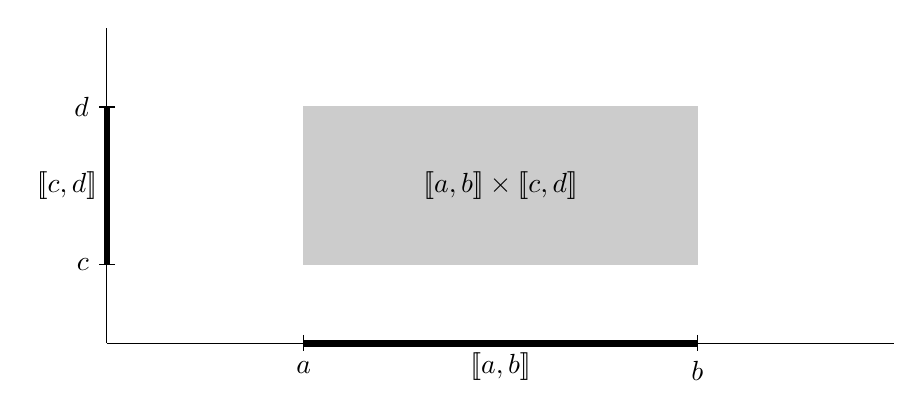
\begin{tikzpicture}[y=1cm, x=2.5cm]	
 	%axis
	\draw(0,0) -- coordinate (x axis mid) (4,0);
    	\draw (0,0) -- coordinate (y axis mid) (0,4);
    	
    	%ticks
    	\draw[fill] (1,1pt) rectangle (3,-1pt);    	
    	\draw (1, 3pt) -- (1, -3pt) node[anchor=north] {$a$};
    	\draw (3, 3pt) -- (3, -3pt) node[anchor=north] {$b$};
    	\draw (2, 0) node[anchor=north] {$[\![a,b]\!]$};
    	
    	\draw[fill] (1pt,1) rectangle (-1pt, 3);
    	\draw (3pt, 1) -- (-3pt, 1) node[anchor=east] {$c$};
    	\draw (3pt, 3) -- (-3pt, 3) node[anchor=east] {$d$};
    	\draw (0,2) node[anchor=east] {$[\![c,d]\!]$};
    	
    	\draw[fill, color=black!20] (1,1) rectangle (3,3);
    	\draw (2, 2) node {$[\![a,b]\!] \times [\![c,d]\!]$ };
\end{tikzpicture}
\end{figure}

\begin{theorem}
	The Cartesian product of a $k$-rectangle in $\mathbb{R}^m$ (where, $k\leq m$) 
	and $\ell$-rectangle in $\mathbb{R}^n$ (again, $\ell \leq n$) 
	is a $(k+\ell)$-rectangle in $\mathbb{R}^{m+n}$.
\end{theorem}

For completeness we will also define a 0-rectangle as a hybrid set containing a single point with multiplicity $1$ or $-1$.
Firstly this allows us to embed $k$-rectangles in $\mathbb{R}^n$.
For example $[\![a,b]\!] \times [\![c,d]\!] \times \hset{e^1}$ is the product of two 1-rectangles and a 0-rectangle (all over $\mathbb{R}$) and so it is a 2-rectangle over $\mathbb{R}^3$.
Specifically, it is the 2-rectangle $[\![a,b]\!] \times [\![c,d]\!]$ on the plane $z=3$.
This also illustrates the principle that given a $k$-rectangle in $\mathbb{R}^n$ where $n>k$ we can always find a $k$ dimensional subspace which also contains the rectangle.
We will re-use the interval notation from earlier although one should be careful to ``type-check'' while interpreting.
When $a$ and $b$ are real numbers then we continue to use the definition $[\![a,b]\!] = [a,b) \ominus [b,a)$.
However, when $\boldsymbol{a}$ and $\boldsymbol{b}$ are $n$-tuples (for example, coordinates in $\mathbb{R}^n$ then this is \emph{not} the oriented line interval $[\boldsymbol{a}, \boldsymbol{b}) \ominus [\boldsymbol{b}, \boldsymbol{a})$.

\begin{definition}
	Let $\boldsymbol{a} = (a_1, a_2, \ldots, a_n)$ and 
	$\boldsymbol{b} = (b_1, b_2, \ldots, b_n)$ be ordered $n$-tuples then we use the notation:
	\begin{align}
		[\![ \boldsymbol{a}, \boldsymbol{b} ]\!] 
		= [\![a_1, b_1]\!] \times [\![a_2, b_2 ]\!] \times \ldots \times [\![a_n , b_n]\!]
	\end{align}
\end{definition}

The dimension of $[\![ \boldsymbol{a}, \boldsymbol{b} ]\!]$ is equal to the number of indices where $a_i$ and $b_i$ are distinct.
For any $i$ where $a_i = b_i$, the corresponding term: $[\![ a_i, b_i ]\!]$ will be a hybrid set containing a single point, that is, a 0-rectangle.
The orientation of $[\![ \boldsymbol{a}, \boldsymbol{b} ]\!]$ is based on the number of negatively oriented intervals $[\![a_i,b_i]\!]$.
Should there be an odd number of indices $i$ such that $a_i > b_i$ then $[\![ \boldsymbol{a}, \boldsymbol{b} ]\!]$ will also be negatively oriented.
Otherwise, it will be positively oriented. 



%%%%%%%%%%%%%%%%%%%%%%%%%%%%%%%%%%%%%%%%%
% Matrix Addition
%%%%%%%%%%%%%%%%%%%%%%%%%%%%%%%%%%%%%%%%%
\section{Matrix Addition}


Now we will consider the addition of $2 \times 2$ block matrices $A$ and $B$ with overall dimensions $n \times m$ 
of the form:
\begin{equation*}
	A = \left[ \begin{array}{cc} A_{11} & A_{12} \\ A_{21} & A_{22} \end{array} \right]
	\;\;\;\;\; \text{and} \;\;\;\;\;
	B = \left[ \begin{array}{cc} B_{11} & B_{12} \\ B_{21} & B_{22} \end{array} \right]
\end{equation*}
Since these are block matrices then $A_{ij}$ and $B_{ij}$ are not entries but sub matrices themselves.
We shall assume that $A_{11}$ is a $(q \times r)$ matrix and $B_{11}$ is a $(s \times t)$ matrix.
The sum of $A$ and $B$ will also be a $n \times m$ matrix.
Our universe, $\mathcal{U}$ is therefore the the set of all indices in an $n \times m$ matrix:
\begin{equation*}
	\mathcal{U} 
		\;=\; [\![0,n)\!)_{\mathbb{N}_0} \times [\![0,m)\!)_{\mathbb{N}_0} 
		\;=\; \{ (i,j) \;|\; 0 \leq i < n \text{ and } 0 \leq j < m \text{ and } i,j \in \mathbb{N}_0 \} 
\end{equation*}


First we must convert $A$ and $B$ to hybrid function notation. 
We will use $\mathcal{A}_{ij}$ an $\mathcal{B}_{ij}$ to respectively denote the regions for which 
$A_{11}$ and $B_{ij}$ are defined.
Explicitly,
\begin{align*}
	&\mathcal{A}_{11} = [\![0,q)\!) \times [\![0,r)\!) &
	\mathcal{A}_{12} = [\![0,q)\!) \times [\![r,m)\!)\;\; &
	\mathcal{A}_{21} = [\![q,n)\!) \times [\![0,r)\!) &
	\mathcal{A}_{22} = [\![q,n)\!) \times [\![r,m)\!) \\
	&\mathcal{B}_{11} = [\![0,s)\!) \times [\![0,t)\!) &
	\mathcal{B}_{12} = [\![0,s)\!) \times [\![t,m)\!)\;\; &
	\mathcal{B}_{21} = [\![s,n)\!) \times [\![0,t)\!) &
	\mathcal{B}_{22} = [\![s,n)\!) \times [\![t,m)\!)
\end{align*}
Which will allow us to rewrite $A$ and $B$ as:
\begin{align*}
	A &= A_{11}^{\mathcal{A}_{11}} \oplus 
		A_{12}^{\mathcal{A}_{12}} \oplus 
		A_{21}^{\mathcal{A}_{21}} \oplus 
		A_{22}^{\mathcal{A}_{22}} \\
	B &= B_{11}^{\mathcal{B}_{11}} \oplus 
		B_{12}^{\mathcal{B}_{12}} \oplus 
		B_{21}^{\mathcal{B}_{21}} \oplus 
		B_{22}^{\mathcal{B}_{22}} 
\end{align*}


Depending on the relation of $q$ with $s$ and $r$ with $t$ the regions in the sum of $A$ and $B$ may vary.
In Figure~\ref{MatAdditionPermutations}, the shapes of block matrices that can arise are shown.
Intuitively, the approach we will take is to not concern ourselves with all possible cases that \emph{could} arise but to just
choose one ordering.
If this ordering is wrong, then the hybrid function multiplicities will handle cancellations to yield the correct expression regardless.


Since there are 4 partitions in $A$ and 4 partitions in $B$, we only require 7 pieces to form a common refinement.
To this refinement for, we follow the same method as in the previous chapter.
\begin{equation}
	\label{eqn:2x2CommonRefinement}
	\mathcal{A}_{11}, \; \mathcal{A}_{12}, \;  \mathcal{A}_{21}, \;
	\mathcal{B}_{11}, \; \mathcal{B}_{12}, \; \mathcal{B}_{21}, \; \mathcal{P}
\end{equation}
where $\mathcal{P}$ is defined as,
$\mathcal{P} = \mathcal{U} 
		\ominus (\mathcal{A}_{11} \oplus \mathcal{A}_{12} \oplus \mathcal{A}_{21} \oplus
				\mathcal{B}_{11} \oplus \mathcal{B}_{12} \oplus \mathcal{B}_{21})$.
Clearly we can still express $\mathcal{A}_{22}$ using only the terms in (\ref{eqn:2x2CommonRefinement}) by
\begin{align*}
	\mathcal{A}_{22} &= \mathcal{U} \ominus (\mathcal{A}_{11} \oplus \mathcal{A}_{12} \oplus \mathcal{A}_{21})\\
		& = \mathcal{U} \ominus (\mathcal{A}_{11} \oplus \mathcal{A}_{12} \oplus \mathcal{A}_{21} \oplus \mathcal{B}_{11} \oplus \mathcal{B}_{12} \oplus \mathcal{B}_{21}) \oplus \mathcal{B}_{11} \oplus \mathcal{B}_{12} \oplus \mathcal{B}_{21}\\
		&= \mathcal{P} \oplus \mathcal{B}_{11} \oplus \mathcal{B}_{12} \oplus \mathcal{B}_{21}
\end{align*}
Similarly $\mathcal{B}_{22}$ can be represented as $\mathcal{B}_{22} = \mathcal{P} \oplus \mathcal{A}_{11} \oplus \mathcal{A}_{12} \oplus \mathcal{A}_{21}$
and $\mathcal{U}$ as the sum of all 7 regions, 
$\mathcal{U} = 	\mathcal{A}_{11} \oplus \mathcal{A}_{12} \oplus \mathcal{A}_{21} \oplus 
				\mathcal{B}_{11} \oplus \mathcal{B}_{12} \oplus \mathcal{B}_{21} \oplus \mathcal{P}$.
Thus $A$ and $B$ can be rewritten using this new generalized partition as:
\begin{align*}
	A &= A_{11}^{\mathcal{A}_{11}} \oplus 
		A_{12}^{\mathcal{A}_{12}} \oplus 
		A_{21}^{\mathcal{A}_{21}} \oplus 
		A_{22}^{\mathcal{P} \oplus \mathcal{B}_{11} \oplus \mathcal{B}_{12} \oplus \mathcal{B}_{21}} \\
	B &= B_{11}^{\mathcal{B}_{11}} \oplus 
		B_{12}^{\mathcal{B}_{12}} \oplus 
		B_{21}^{\mathcal{B}_{21}} \oplus 
		B_{22}^{\mathcal{P} \oplus \mathcal{A}_{11} \oplus \mathcal{A}_{12} \oplus \mathcal{A}_{21}} 
\end{align*}

And addition becomes straightforward. 
We add functions for terms over corresponding regions.
Since we are using \emph{generalized partitions}, not traditional partitions we cannot guarantee disjointness.
As such we must also apply a $+$-reduction after summing each matching pair:
\begin{align*}
	(A+B) = \R[+] & \left(  (A_{11}+B_{22})^{\mathcal{A}_{11}} \oplus 
		(A_{12} + B_{22})^{\mathcal{A}_{12}} \oplus 
		(A_{21} + B_{22})^{\mathcal{A}_{21}} \right. \\ &\oplus 
		(A_{22} + B_{11})^{\mathcal{B}_{11}} \oplus 
		(A_{22} + B_{12})^{\mathcal{B}_{12}} \oplus 
		(A_{22} + B_{21})^{\mathcal{B}_{21}} \\ &\oplus
		\left.(A_{22} + B_{22})^{\mathcal{P}} \right)
\end{align*}


\todo[inline]{Evaluating at points}


This extends easily to addition of more complex block matrices as well.
If we consider conformable matrices $A$ and $B$ of the form:

\begin{equation*}
	A = \begin{bmatrix}
		A_{11} & \ldots & A_{1\ell}\\
		\vdots & & \vdots \\
		A_{k1} & \ldots & A_{k\ell}	
	\end{bmatrix}
	\;\;\;\;\;
	\text{ and }
	\;\;\;\;\;
	B = \begin{bmatrix}
		B_{11} & \ldots & B_{1m}\\
		\vdots & & \vdots \\
		B_{n1} & \ldots & B_{nm}	
	\end{bmatrix}
\end{equation*}
For  sequences $q$, $r$, $s$, and $t$ which are strictly increasing and additionally constrained by 
${q_0 = r_0 = s_0 = t_0 = 0}$ and $q_k = s_n$ and $r_\ell = t_m$.
Each $A_{ij}$ and $B_{ij}$ is defined over a rectangular region $\mathcal{A}_{ij}$ and $\mathcal{B}_{ij}$:
 \begin{equation*}
	\mathcal{A}_{ij} = [\![q_{i-1}, q_i )\!) \times [\![ r_{j-1}, r_{j} )\!)
	\;\;\;\;\;
	\mathcal{B}_{ij} = [\![s_{i-1}, s_i )\!) \times [\![ t_{j-1}, t_{j} )\!)
\end{equation*}
which gives the expression:
\begin{equation}
	(A+B) = \R[+] \left( 
		\left( \bigoplus_{(i,j) \neq (n,m)} (A_{ij} + B_{nm})^{\mathcal{A}_{ij}} \right) \oplus
		\left( \bigoplus_{(i,j) \neq (n,m)} (A_{nm} + B_{ij})^{\mathcal{B}_{ij}} \right) \oplus
			(A_{nm} + B_{nm})^{\mathcal{P}} 
	\right)
\end{equation}




%%%%%%%%%%%%%%%%%%%%%%%%%%%%%%%%%%%%%%%%%
% Matrix Multiplication
%
% q = k1, r = q2, s = ell1, t=ell2
%%%%%%%%%%%%%%%%%%%%%%%%%%%%%%%%%%%%%%%%%
\section{Matrix Multiplication}


Next we will consider the product of symbolic block matrices.
Again, we will assume $2 \times 2$ block matrices $A$ and $B$.
However for these matrices to be conformable for multiplication they must be  $n \times m$ and $m \times p$ rather than
the same size as was required for addition.
\begin{equation}
	A = \begin{bmatrix} A_{11} & A_{12} \\ A_{21} & A_{22} \end{bmatrix}
	\;\;\;\;\; \text{and} \;\;\;\;\;
	B = \begin{bmatrix} B_{11} & B_{12} \\ B_{21} & B_{22} \end{bmatrix}
\end{equation}
Where $A_{11}$ is a $q \times r$ matrix and $B_{11}$ is a $s \times t$ matrix.
Note that $0 \leq r , s \leq m$ but the ordering of $r$ and $s$ is unknown.


In the simplest case, $r=s$, four regions will arise each with simple closed expressions. 
\begin{equation}
	AB = \begin{bmatrix}
		\left( A_{11}B_{11}+A_{12}B_{21} \right) & \left( A_{11}B_{12}+A_{12}B_{22} \right) \\ 
		\left( A_{21}B_{11}+A_{22}B_{21} \right) & \left( A_{21}B_{12}+A_{22}B_{22} \right)
	\end{bmatrix}
\end{equation}
One should notice the similarity between this and multiplication of simple $2 \times 2$ matrices.
If we consider only the top-left block, since $r=s$ then the $(q \times r)$ matrix $A_{11}$ and the 
$(s \times t)$ matrix $B_{11}$ are conformable.
As are the $(q \times m-r)$ matrix $A_{12}$ and the $(m-s \times t)$ matrix $B_{21}$.
Both products will result in a $q \times t$ matrix which are conformable for addition.
Thus the term $A_{11}B_{11} + A_{12}B_{21}$ is a $q \times t$ block. 


If $r \neq s$ then one approach would be to partition $A$ into a $2 \times 3$ block matrix 
split along the vertical lines $r$ and $s$ and the horizontal line $q$.
And split $B$ into a $3 \times 2$ block matrix split along the vertical line $t$  and the horizontal lines $r$ and $s$:
Depending on the relative ordering of $r$ and $s$ this may cause different blocks to be split.
If $s < r$ then $A_{11}$ and $A_{21}$ will be split into blocks with columns from 0 to $s$ and then from $s$ to $r$
while $B_{21}$ and $B_{22}$ would be split into blocks with rows from $s$ to $r$ and from $r$ to $m$.
\begin{equation*}
	A= \left[ \begin{array}{cc|c}
			A_{11}^{(1)} & A_{11}^{(2)} & A_{12}^{} \\ 
			\hline
			A_{21}^{(1)} & A_{21}^{(2)} & A_{22}^{}
		\end{array} \right]
	\;\;\;\;\;\text{and}\;\;\;\;\;
	B = \left[ \begin{array}{c|c}
			B_{11}^{} & B_{12}^{} \\
			\hline
			B_{21}^{(1)} & B_{22}^{(1)} \\
			B_{21}^{(2)} & B_{22}^{(2)} 
		\end{array} \right]
\end{equation*}


The resulting product is still a $2 \times 2$ matrix.
Additionally, each block is still the same size; the first block in the top-left is still $q \times t$.
However each block is now the sum of three block products:
\begin{equation*}
	AB 	= 	\begin{bmatrix}
				\left( A_{11}^{(1)}B_{11}^{}+ A_{11}^{(2)}B_{21}^{(1)} + A_{12}^{}B_{21}^{(2)} \right) & 
				\left( A_{11}^{(1)}B_{12}^{}+ A_{11}^{(2)}B_{22}^{(1)} + A_{12}^{}B_{22}^{(2)} \right) \\
				\left( A_{21}^{(1)}B_{11}^{}+ A_{21}^{(2)}B_{21}^{(1)} + A_{22}^{}B_{21}^{(2)} \right) & 
				\left( A_{21}^{(1)}B_{12}^{}+ A_{21}^{(2)}B_{22}^{(1)} + A_{22}^{}B_{22}^{(2)} \right) 
			\end{bmatrix}
\end{equation*}
On the other hand, if $r < s$ then $A_{12}$ and $A_{22}$ will be the blocks split vertically while $B_{11}$ and $B_{12}$
will be split horizontally. 
In turn, this leads to a different expression for the product of $A$ and $B$.
In a now familiar, pattern we can use hybrid functions to give a single expression to deal with all permutations simultaneously.



First we shall refer to the product $AB$ by the block matrix $C$:
\begin{equation}
	AB = C = \begin{bmatrix} C_{11} & C_{12} \\ C_{21} & C_{22} \end{bmatrix}
\end{equation}
$C$ is an $n \times p$ matrix as determined by the sizes of $A$ and $B$ and $C_{11}$ is a $q \times t$ sub-matrix.
This leaves $C_{12}$, $C_{21}$ and $C_{22}$ to be $q \times (p-t)$, $(n-q) \times t$ and $(n-q) \times (p-t)$ respectively.
We will partition all three matrices along the axes $0.. n$, $0..p$ and $0..m$ into the oriented intervals:
\begin{equation*}\begin{array}{cc}
	N_1 = [\![0, q)\!) & N_2 = [\![q, n)\!) 
\end{array}\end{equation*}
\begin{equation*}\begin{array}{cc}
	P_1 = [\![0, t)\!) & P_2 = [\![t, p)\!)
\end{array}\end{equation*}
\begin{equation*}\begin{array}{ccc}
	M_1 = [\![0, r)\!) & M_2 = [\![r, s)\!) & M_3 = [\![s, m)\!)
\end{array}\end{equation*}


Assumption is too strong a word, but these partitions follow the \emph{guess} that $r<s$.
So we will be constructing expressions with this in mind. 
If we chose incorrectly, then we plan to use the negative orientation of $M_2$ to correct our expression.
Using these intervals, we can now rewrite our matrices inline as:
\begin{align}
	A & =	A_{11}^{N_1 \times M_1} \oplus A_{12}^{N_1 \times (M_2 \oplus M_3)} \oplus 
			A_{21}^{N_2 \times M_1} \oplus A_{22}^{N_2 \times (M_2 \oplus M_3)} \\
	B & =	B_{11}^{(M_1 \oplus M_2) \times P_1} \oplus B_{12}^{(M_1 \oplus M_2) \times P_2} \oplus 
			B_{21}^{M_3 \times P_1} \oplus B_{12}^{M_3 \times P_2}\\
	C & =	C_{11}^{N_1 \times P_1} \oplus C_{12}^{N_1 \times P_2} \oplus
			C_{21}^{N_2 \times P_1} \oplus C_{22}^{N_2 \times P_2}
\end{align}
It should be noted here that $\oplus$ is still the point-wise sum of hybrid functions.
It should not be confused with the direct sum or Kronecker sum of matrices which both use the same $\oplus$ operator.
The $\times$ operator refers to the Cartesian product of intervals. 

For $i,j \in \{ 1,2 \}$ the terms of $C$ are given by.
\begin{equation}
	C_{i,j} 	= A_{i,1}^{N_i \times M_1} B_{1,j}^{M_1 \times P_j} 
			+ A_{i,2}^{N_i \times M_2} B_{1,j}^{M_2 \times P_j}
			+ A_{i,2}^{N_i \times M_3} B_{2,j}^{M_3 \times P_j}
\end{equation}

If $r=s$ then $M_2 = \emptyset$.
We can think of multiplying a $n \times 0$ matrix by a $0 \times p$ matrix as giving a $n \times p$ matrix which is the sum
over an empty set, 0 everywhere.
If $r < s$ then this is like treating $A$ and $B$ instead as $2 \times 3$ and $3 \times 2$ block matrices.
$M_1$, $M_2$ and $M_3$ are all positive intervals and form conformable blocks.

If $r > s$ then $M_2$ is a negative interval.
The product $A_{i,2}^{N_i \times M_2} B_{1,j}^{M_2 \times P_j}$ may be symbolically conformable but it begs the 
question of what exactly a $(2 \times -3)$ or $(-1 \times 4)$ matrix would even look like.
To simplify $C_{i,j}$, we can use the generalized partition:
\begin{equation*}
 	\Big\{ \left(M_1 \oplus M_2\right), \;\; \ominus M_2, \;\; \left(M_2 \oplus M_3\right) \Big\}
\end{equation*}
which contains only positive oriented intervals.
Now we can split the first and third terms using $M_1 = (M_1 \oplus M_2) \ominus M_2$ 
and $M_3 = \ominus M_2 \oplus (M_2 \oplus M_3)$:
\begin{align*}
	C_{i,j} 	= &\left( A_{i,1}^{N_i \times M_1 \oplus M_2} \oplus A_{i,1}^{N_i \times \ominus M_2} \right)
				\left( B_{1,j}^{M_1 \oplus M_2 \times P_j} \oplus B_{1,j}^{\ominus M_2 \times P_j} \right)
			+ A_{i,2}^{N_i \times M_2} B_{1,j}^{M_2 \times P_j} \notag\\
			&+ \left( A_{i,2}^{N_i \times \ominus M_2} \oplus A_{i,2}^{N_i \times M_3 \oplus M_2} \right)
			 \left( B_{2,j}^{\ominus M_2 \times P_j} \oplus B_{2,j}^{M_3 \oplus M_2 \times P_j} \right)
\end{align*}

These resulting hybrid function sums are themselves inline block matrices!
The products, $\left( A_{i,1}^{N_i \times M_1 \oplus M_2} \oplus A_{i,1}^{N_i \times \ominus M_2} \right)
	  \left( B_{1,j}^{M_1 \oplus M_2 \times P_j} \oplus B_{1,j}^{\ominus M_2 \times P_j} \right)$
and $\left( A_{i,1}^{N_i \times M_1 \oplus M_2} \oplus A_{i,1}^{N_i \times \ominus M_2} \right)
	  \left( B_{1,j}^{M_1 \oplus M_2 \times P_j} \oplus B_{1,j}^{\ominus M_2 \times P_j} \right)$	 
are each conformable $1 \times 2$ and $2 \times 1$ block matrices.
Their product is a $1 \times 1$ block matrix given by a sum of two $N_i \times P_j$ matrices.
\begin{align*}
	C_{i,j} 	= & \left( A_{i,1}^{N_i \times M_1 \oplus M_2} B_{1,j}^{M_1 \oplus M_2 \times P_j}
			+ A_{i,1}^{N_i \times \ominus M_2} B_{1,j}^{\ominus M_2 \times P_j} \right)
			+ A_{i,2}^{N_i \times M_2} B_{1,j}^{M_2 \times P_j} \notag\\
			&+ \left( A_{i,2}^{N_i \times \ominus M_2} B_{2,j}^{\ominus M_2 \times P_j}
			+ A_{i,2}^{N_i \times M_3 \oplus M_2} B_{2,j}^{M_3 \oplus M_2 \times P_j} \right)
\end{align*}

Rearranging the braces, we can recombine the middle three terms to form the product of $1 \times 3$ and $3 \times 1$ block matrices:
\begin{align*}
	C_{i,j} 	=& \left( A_{i,1}^{N_i \times \ominus M_2} 
				\oplus  A_{i,2}^{N_i \times M_2} 
				\oplus A_{i,2}^{N_i \times \ominus M_2} \right)
			\left( B_{1,j}^{\ominus M_2 \times P_j} 
				\oplus B_{1,j}^{M_2 \times P_j} 
				\oplus B_{2,j}^{\ominus M_2 \times P_j} \right)\notag\\
			&+ A_{i,1}^{N_i \times M_1 \oplus M_2} B_{1,j}^{M_1 \oplus M_2 \times P_j} 
			+ A_{i,2}^{N_i \times M_3 \oplus M_2} B_{2,j}^{M_3 \oplus M_2 \times P_j} 
\end{align*}
But the term $A_{i,2}$ occurs twice; once over $N_i \times M_2$ and once over $N_i \times \ominus M_2$.
As hybrid functions with the same corresponding function, we can combine them by $f^A \oplus f^B = f^{A\oplus B}$.
But the regions only differ by a sign and sum to the empty set.
Similarly, the $B_{1,j}$ terms also cancel:
\begin{align*}
	C_{i,j} 	=& \left( A_{i,1}^{N_i \times \ominus M_2} \oplus  A_{i,2}^{N_i \times \emptyset}  \right)
			\left(  B_{2,j}^{\ominus M_2 \times P_j} \oplus B_{1,j}^{\emptyset \times P_j} \right)\notag\\
			&+ A_{i,1}^{N_i \times M_1 \oplus M_2} B_{1,j}^{M_1 \oplus M_2 \times P_j} 
			+ A_{i,2}^{N_i \times M_3 \oplus M_2} B_{2,j}^{M_3 \oplus M_2 \times P_j} 
\end{align*}
And finally cleaning up this expression by removing the terms over empty regions gives us the desired:
\begin{equation}
	C_{i,j} =  A_{i,1}^{N_i \times M_1 \oplus M_2} B_{1,j}^{M_1 \oplus M_2 \times P_j} 
			+ A_{i,1}^{N_i \times \ominus M_2} B_{2,j}^{\ominus M_2 \times P_j}
			+ A_{i,2}^{N_i \times M_3 \oplus M_2} B_{2,j}^{M_3 \oplus M_2 \times P_j}
\end{equation}





\todo[inline]{example}

\todo[inline]{multiple blocks}
 
\todo[inline]{wrap-up}













